% !TeX root = Chapter_01_Slides.tex
% Chapter 1 lecture slides — Why Risk Management Matters
% Pilot deck for the instructor-resource series.
\documentclass[11pt, aspectratio=169]{beamer}
\usepackage{tikz}
\makeatletter
\def\input@path{{./}{../slides/}}
\makeatother
\usepackage{erm_beamer_theme}
\usepackage{amsmath,amssymb}
\graphicspath{{../rscripts/chapter1/jnj_tylenol/}}

\title[ERM Ch.\,1]{Why Risk Management Matters}
\subtitle{Enterprise Risk Management, Second Edition --- Chapter 1}
\author{Martin F.\ Grace}
\institute{University of Iowa\\[2pt] Tippie College of Business\\[2pt] Vaughan Institute of Risk Management}
\date{June 2026}

\begin{document}

\begin{frame}[plain]
\titlepage
\end{frame}

\begin{frame}{Learning Objectives}
\begin{itemize}
  \item Explain why corporate risk management appears \alert{irrelevant} under perfect-market assumptions.
  \item Identify the assumptions behind the Modigliani--Miller propositions and the CAPM.
  \item Evaluate how taxes, distress costs, agency problems, information asymmetry, and regulation make risk management valuable.
  \item Define the \alert{cost of risk} and explain why minimizing it is not the same as eliminating risk.
  \item Apply the chapter's logic to a corporate crisis where reputation, safety, and financial value interact.
\end{itemize}
\end{frame}

\section{Opening Case: The Tylenol Murders}

\begin{frame}{September 29, 1982}
\begin{itemize}
  \item Seven people in the Chicago area die after taking Extra-Strength Tylenol capsules laced with potassium cyanide.
  \item Tampering occurred \emph{on store shelves} --- bottles opened, capsules replaced, returned.
  \item Tylenol at the time: $\sim$35\% of the OTC pain reliever market, close to a fifth of J\&J's corporate profits.
  \item No one knew how many bottles were poisoned, or where.
\end{itemize}
\medskip
\begin{block}{The decision problem}
Every option was costly, the facts were incomplete, and the clock was running. What would \emph{you} have done by October 5?
\end{block}
\end{frame}

\begin{frame}{Johnson \& Johnson's Response}
\begin{columns}[T]
\column{0.48\textwidth}
\textbf{Week one}
\begin{itemize}
  \item October 5: nationwide recall --- 31 million bottles, $>$\$100M retail value (1982 dollars)
  \item Advertising halted; toll-free hotlines; full cooperation with FDA, FBI, police
\end{itemize}
\column{0.48\textwidth}
\textbf{The rebuild}
\begin{itemize}
  \item November 1982: triple-sealed, tamper-resistant packaging
  \item Education campaigns, discounts to win customers back
  \item Within a few years: market leadership regained
\end{itemize}
\end{columns}
\medskip
The murders remain unsolved. The response became the canonical example of crisis management.
\end{frame}

\begin{frame}{The Market's Verdict}
\begin{columns}[T]
\column{0.62\textwidth}
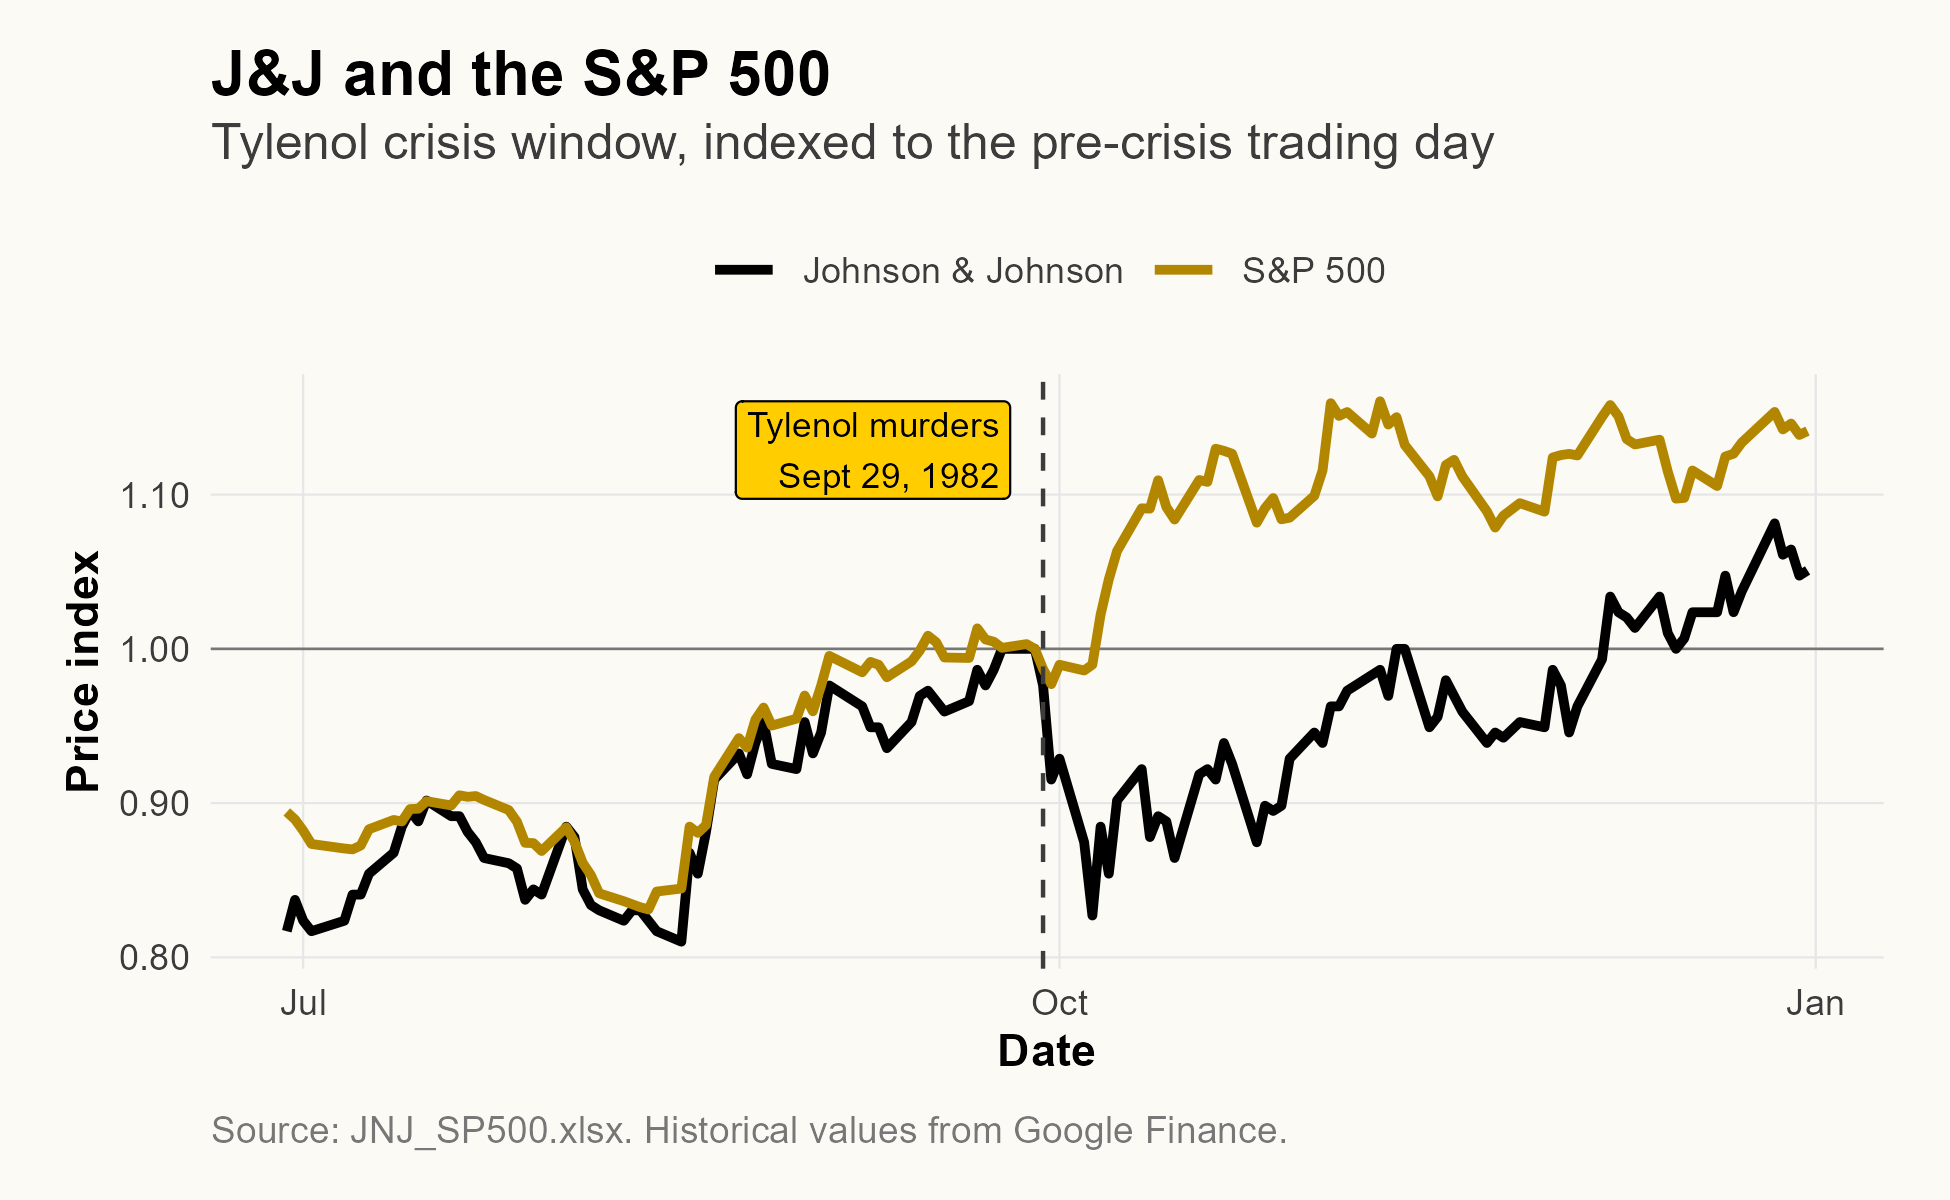
\includegraphics[width=\textwidth]{c1_jnjplot.png}
\column{0.34\textwidth}
\begin{itemize}
  \item Sharp drop below the S\&P 500 after September 29
  \item Recovery to roughly pre-crisis relative value by December 1982
  \item Costly --- but the recall, communication, and redesign restored confidence within \emph{two months}
\end{itemize}
\end{columns}
\end{frame}

\section{The Paradox of Risk Management}

\begin{frame}{The Paradox}
\begin{itemize}
  \item Firms spend billions on insurance, hedging, CROs, and board risk committees.
  \item Yet finance theory says: under idealized conditions, none of this should affect firm value.
  \item If shareholders can diversify away firm-specific risk on their own, why should the \emph{firm} spend money managing it?
\end{itemize}
\medskip
\begin{block}{Resolving the paradox}
In theory, risk management shouldn't matter. In practice, it clearly does.
The answer lies in the \alert{frictions} the theory assumes away --- each one is a
potential source of value for risk management.
\end{block}
\end{frame}

\section{The Benchmark: Irrelevance in Perfect Markets}

\begin{frame}{Modigliani--Miller (1958)}
\begin{itemize}
  \item Under idealized assumptions, firm value is independent of capital structure --- and, by extension, of dividend policy and risk management.
  \item Intuition: investors can \alert{replicate or undo} any financial decision the firm makes.
  \begin{itemize}
    \item Firm too conservative? Borrow personally to add leverage.
    \item Firm too levered? Lend at the risk-free rate to offset.
  \end{itemize}
  \item Value is determined by \emph{real assets and investment opportunities}, not by how cash flows are packaged.
\end{itemize}
\end{frame}

\begin{frame}{The CAPM}
\[
E[R_i] = R_f + \beta_i \left( E[R_M] - R_f \right)
\]
\begin{itemize}
  \item Only \alert{systematic risk} (beta) is priced in equilibrium.
  \item \alert{Idiosyncratic risk} is eliminated by holding a diversified portfolio --- investors are not compensated for bearing it.
\end{itemize}
\medskip
\begin{block}{Implication for the firm}
Insuring the plant against fire, hedging firm-specific commodity exposure, spending on loss control: none of it reduces systematic risk, so none of it lowers the cost of capital --- in the CAPM world.
\end{block}
\end{frame}

\begin{frame}{What Irrelevance Means --- and Doesn't}
\begin{itemize}
  \item Irrelevance $\neq$ ``risk doesn't matter.'' It means risk management is \alert{redundant}: shareholders can replicate it at zero cost.
  \begin{itemize}
    \item Firm hedges interest rates? Shareholder takes an offsetting derivative position.
    \item Firm buys fire insurance? A diversified portfolio already averages away fire risk.
    \item Firm smooths earnings? Investors see through to the underlying cash flows.
  \end{itemize}
  \item The benchmark isolates the real question:
\end{itemize}
\medskip
\begin{center}
\large\emph{What conditions must fail for risk management to add value?}
\end{center}
\end{frame}

\begin{frame}{The Assumptions Doing the Work}
\begin{columns}[T]
\column{0.48\textwidth}
\begin{itemize}
  \item Frictionless markets (no transaction costs, taxes)
  \item Homogeneous expectations
  \item Mean--variance preferences
  \item Unlimited borrowing/lending at $R_f$
\end{itemize}
\column{0.48\textwidth}
\begin{itemize}
  \item All risks tradable
  \item Perfect, symmetric information
  \item No bankruptcy or distress costs
  \item No agency conflicts
  \item Investment policy independent of financing
\end{itemize}
\end{columns}
\medskip
Each assumption that fails in the real world is a candidate explanation for why firms manage risk.
\end{frame}

\section{Seven Frictions That Make Risk Management Matter}

\begin{frame}{Friction 1: Tax Convexity}
\begin{itemize}
  \item Real tax schedules are convex: progressive rates, limited loss offsets, expiring carryforwards.
  \item Jensen's inequality: with a convex tax function, \alert{volatile income pays more expected tax} than stable income with the same mean.
\end{itemize}
\medskip
\begin{exampleblock}{Example: 20\% below \$100M, 30\% above}
\begin{itemize}
  \item Firm A (stable): \$100M every year $\Rightarrow$ tax \$20M
  \item Firm B (volatile): \$50M or \$150M, same mean $\Rightarrow$ average tax \$22.5M
  \item Volatility alone costs Firm B \alert{\$2.5M per year}. Smoothing income recovers it.
\end{itemize}
\end{exampleblock}
\end{frame}

\begin{frame}{Friction 2: Costly Financial Distress}
\[
\text{Expected Distress Cost} = \Pr(\text{Distress}) \times \text{Cost if Distressed}
\]
\begin{itemize}
  \item \textbf{Direct costs}: legal, court, advisory fees --- roughly 3--5\% of firm value.
  \item \textbf{Indirect costs}: customers flee, suppliers tighten terms, talent leaves --- can exceed 10--20\% of pre-distress value.
  \item Volatility raises $\Pr(\text{Distress})$; hedging, insurance, and liquidity buffers lower it.
  \item Benefit is largest for leveraged firms and reputation-sensitive industries.
\end{itemize}
\end{frame}

\begin{frame}{Friction 3: Underinvestment}
\begin{itemize}
  \item External capital is costly or unavailable exactly when internal funds run short.
  \item Volatile cash flows mean the firm may be cash-poor when good projects appear --- and the NPV is lost.
\end{itemize}
\medskip
\begin{exampleblock}{Example: a \$50M project}
\begin{itemize}
  \item Cash flow \$30M or \$70M with equal probability; no external finance.
  \item Unhedged: project funded only half the time --- half the NPV lost.
  \item Hedged to \$50M in both states: funded \emph{always}. Risk management preserves the option to invest.
\end{itemize}
\end{exampleblock}
\end{frame}

\begin{frame}{Friction 4: Agency Problems}
\begin{itemize}
  \item Managers can't diversify their human capital or firm-tied compensation $\Rightarrow$ often \alert{more risk-averse} than shareholders.
  \item Option-heavy pay can flip the problem: \alert{excessive} risk-taking (``gambling for resurrection'').
  \item Risk management helps both ways:
  \begin{itemize}
    \item Hedge the risks that frighten managers but don't matter to diversified shareholders --- freeing managers to take good strategic risks.
    \item Risk limits and board oversight constrain the gamblers.
    \item Smoother performance signals make incentive contracts work better.
  \end{itemize}
\end{itemize}
\end{frame}

\begin{frame}{Friction 5: Information Asymmetry}
\begin{itemize}
  \item Managers know more than investors $\Rightarrow$ adverse selection premium, possible undervaluation, opaque earnings.
  \item Risk management responds by:
  \begin{itemize}
    \item \textbf{Smoothing noise}: hedged earnings reveal operating performance, not commodity luck.
    \item \textbf{Signaling}: a consistent hedging policy is a credible signal of quality and long-term orientation.
    \item \textbf{Lowering the cost of capital}: less uncertainty about quality, smaller premium demanded.
  \end{itemize}
\end{itemize}
\end{frame}

\begin{frame}{Frictions 6 \& 7: Stakeholders and Regulators}
\begin{columns}[T]
\column{0.48\textwidth}
\textbf{Stakeholder relationships}
\begin{itemize}
  \item Employees, customers, suppliers are \emph{not} diversified in the firm.
  \item Volatility makes them demand compensation: higher wages, worse terms, lost sales.
  \item Stability lowers contracting costs and protects implicit commitments.
\end{itemize}
\column{0.48\textwidth}
\textbf{Regulation and ratings}
\begin{itemize}
  \item Banks and insurers face risk-based capital rules; breaches are expensive.
  \item Rating agencies penalize volatility; ratings drive borrowing costs.
  \item Example: reinsurance stabilizes surplus $\Rightarrow$ better rating $\Rightarrow$ more business at better terms.
\end{itemize}
\end{columns}
\end{frame}

\section{The Cost of Risk}

\begin{frame}{A Unifying Framework}
\[
\begin{aligned}
\text{Cost of Risk} ={}& \text{Expected Retained Losses} + \text{Risk Control Costs} \\
&+ \text{Risk Financing Costs} + \text{Indirect Costs of Volatility}
\end{aligned}
\]
\begin{itemize}
  \item The indirect costs are the seven frictions: taxes, distress, underinvestment, agency, information, stakeholders, regulation.
  \item The goal is \alert{not} to eliminate risk --- risk is inseparable from return.
\end{itemize}
\medskip
\begin{block}{The objective of corporate risk management}
Minimize the \emph{total} cost of risk, subject to the firm's strategic goals and risk appetite. Manage a risk when the reduction in indirect costs exceeds the direct cost of managing it.
\end{block}
\end{frame}

\begin{frame}{Risk Management Is Core Corporate Finance}
\begin{itemize}
  \item Not a specialized silo: every major decision --- capital structure, investment, hedging --- changes the cost of risk.
  \item Done well, it frees capital, preserves flexibility to invest, aligns incentives, and lowers the cost of capital.
  \item Back to Tylenol: J\&J's recall was ``irrational'' in a perfect-market world. In the real world --- reputation, stakeholders, regulation --- it protected the franchise and restored value within two months.
\end{itemize}
\end{frame}

\begin{frame}{Discussion Questions}
\begin{enumerate}
  \item In the MM/CAPM world, J\&J's \$100M recall destroys value. Which frictions made it value-\emph{creating} in 1982?
  \item Why might a small, family-owned firm rationally buy more insurance than a large public company with the same risks?
  \item A CFO says: ``We hedge to smooth earnings because analysts hate surprises.'' Which friction(s) is she invoking --- and is the argument sound?
  \item Give an example of a risk a firm should \emph{retain}, and explain why using the cost-of-risk framework.
\end{enumerate}
\end{frame}

\end{document}
